\documentclass[12pt]{article}
% include packages
\usepackage[margin=1in]{geometry} 
\usepackage[shortlabels]{enumitem}
\usepackage{caption}
\usepackage{algorithm}
\usepackage[noend]{algpseudocode}
\usepackage[table,xcdraw]{xcolor}
\usepackage{import}
\usepackage{tikz}
\usepackage{tikz,fullpage}
\usetikzlibrary{arrows, automata}
\usepackage{tkz-berge}
\usepackage[position=top]{subfig}
\usepackage{amsmath,amsthm,amssymb,amsfonts, enumitem, fancyhdr, color, comment, graphicx, environ}
% styling
\pagestyle{fancy}
\setlength{\headheight}{65pt}
\newenvironment{problem}[2][Problem]{\begin{trivlist}
\item[\hskip \labelsep {\bfseries #1}\hskip \labelsep {\bfseries #2.}]}{\end{trivlist}}
\newenvironment{sol}
    {\emph{Solution:}
    }
    {
    \qed
    }
\specialcomment{com}{ \color{blue} \textbf{Comment:} }{\color{black}} %for instructor comments while grading
\NewEnviron{probscore}{\marginpar{ \color{blue} \tiny Problem Score: \BODY \color{black} }}

% creates keywords for input and output in algorithm block
\algblock{Input}{EndInput}
\algnotext{EndInput}
\algblock{Output}{EndOutput}
\algnotext{EndOutput}
\newcommand{\Desc}[2]{\State \makebox[13em][l]{#1}#2}

% ------------- Header Information ------------- 
\def \FirstLastName{John Doe}
\def \UserID{doejohn}
\def \CourseNumber{CS 101}
\def \SectionNumber{Section 001}
\def \Term{Winter 2019}
\def \AssignmentTitle{HW 1}
% ---------------------------------------------- 

% Header
\lhead{\FirstLastName{} \textit{(\UserID{})}}
\rhead{\CourseNumber{} \\ \SectionNumber{} \\ \Term{} \\ \AssignmentTitle{}}

\begin{document}
% include problems tex files
\begin{problem}{1: Title} Question details
\end{problem}
\begin{sol}
Answer
\end{sol}
\subsection{Held-Karp Algorithm (Dynamic Algorithm)}
\subsubsection{Run-time Analysis}
$O(n^2 * 2^n)$
\subsubsection{Code}

% add programming code
\import{code/}{code.tex}

\subsubsection{Description}
Lorem ipsum dolor sit amet, ea putent ceteros eam, duo ne lorem vidisse quaestio. Te dolor eleifend adolescens vis. Mea vivendum neglegentur cu. Vel ad nobis corrumpit percipitur, eam zril nonumy corpora id. Pro inani voluptua omittantur id, ne ipsum harum eos. Magna aeque consul at cum, ei melius definitiones usu.

Nam ea odio tollit iuvaret, bonorum persecuti mel ex. Ancillae phaedrum erroribus vis ne. Prima ullum propriae et per, brute aliquam inermis ad nam. Nam unum veri nostrud ex, nemore fabellas conceptam cum ad. Vis ut discere ullamcorper.

Eu voluptua vituperata eum, no alii epicuri has. Vis magna utinam disputationi an. Probo feugait forensibus sea no, saperet perpetua splendide no pri, in nemore nominati vis. An sed aliquam iudicabit, harum feugait usu id, cu ius tota everti. Ne eripuit minimum pri, est te stet pertinax, aliquam noluisse iracundia et eos.

\newpage

% include images/code snippets
\begin{figure}[h]
\begin {center}
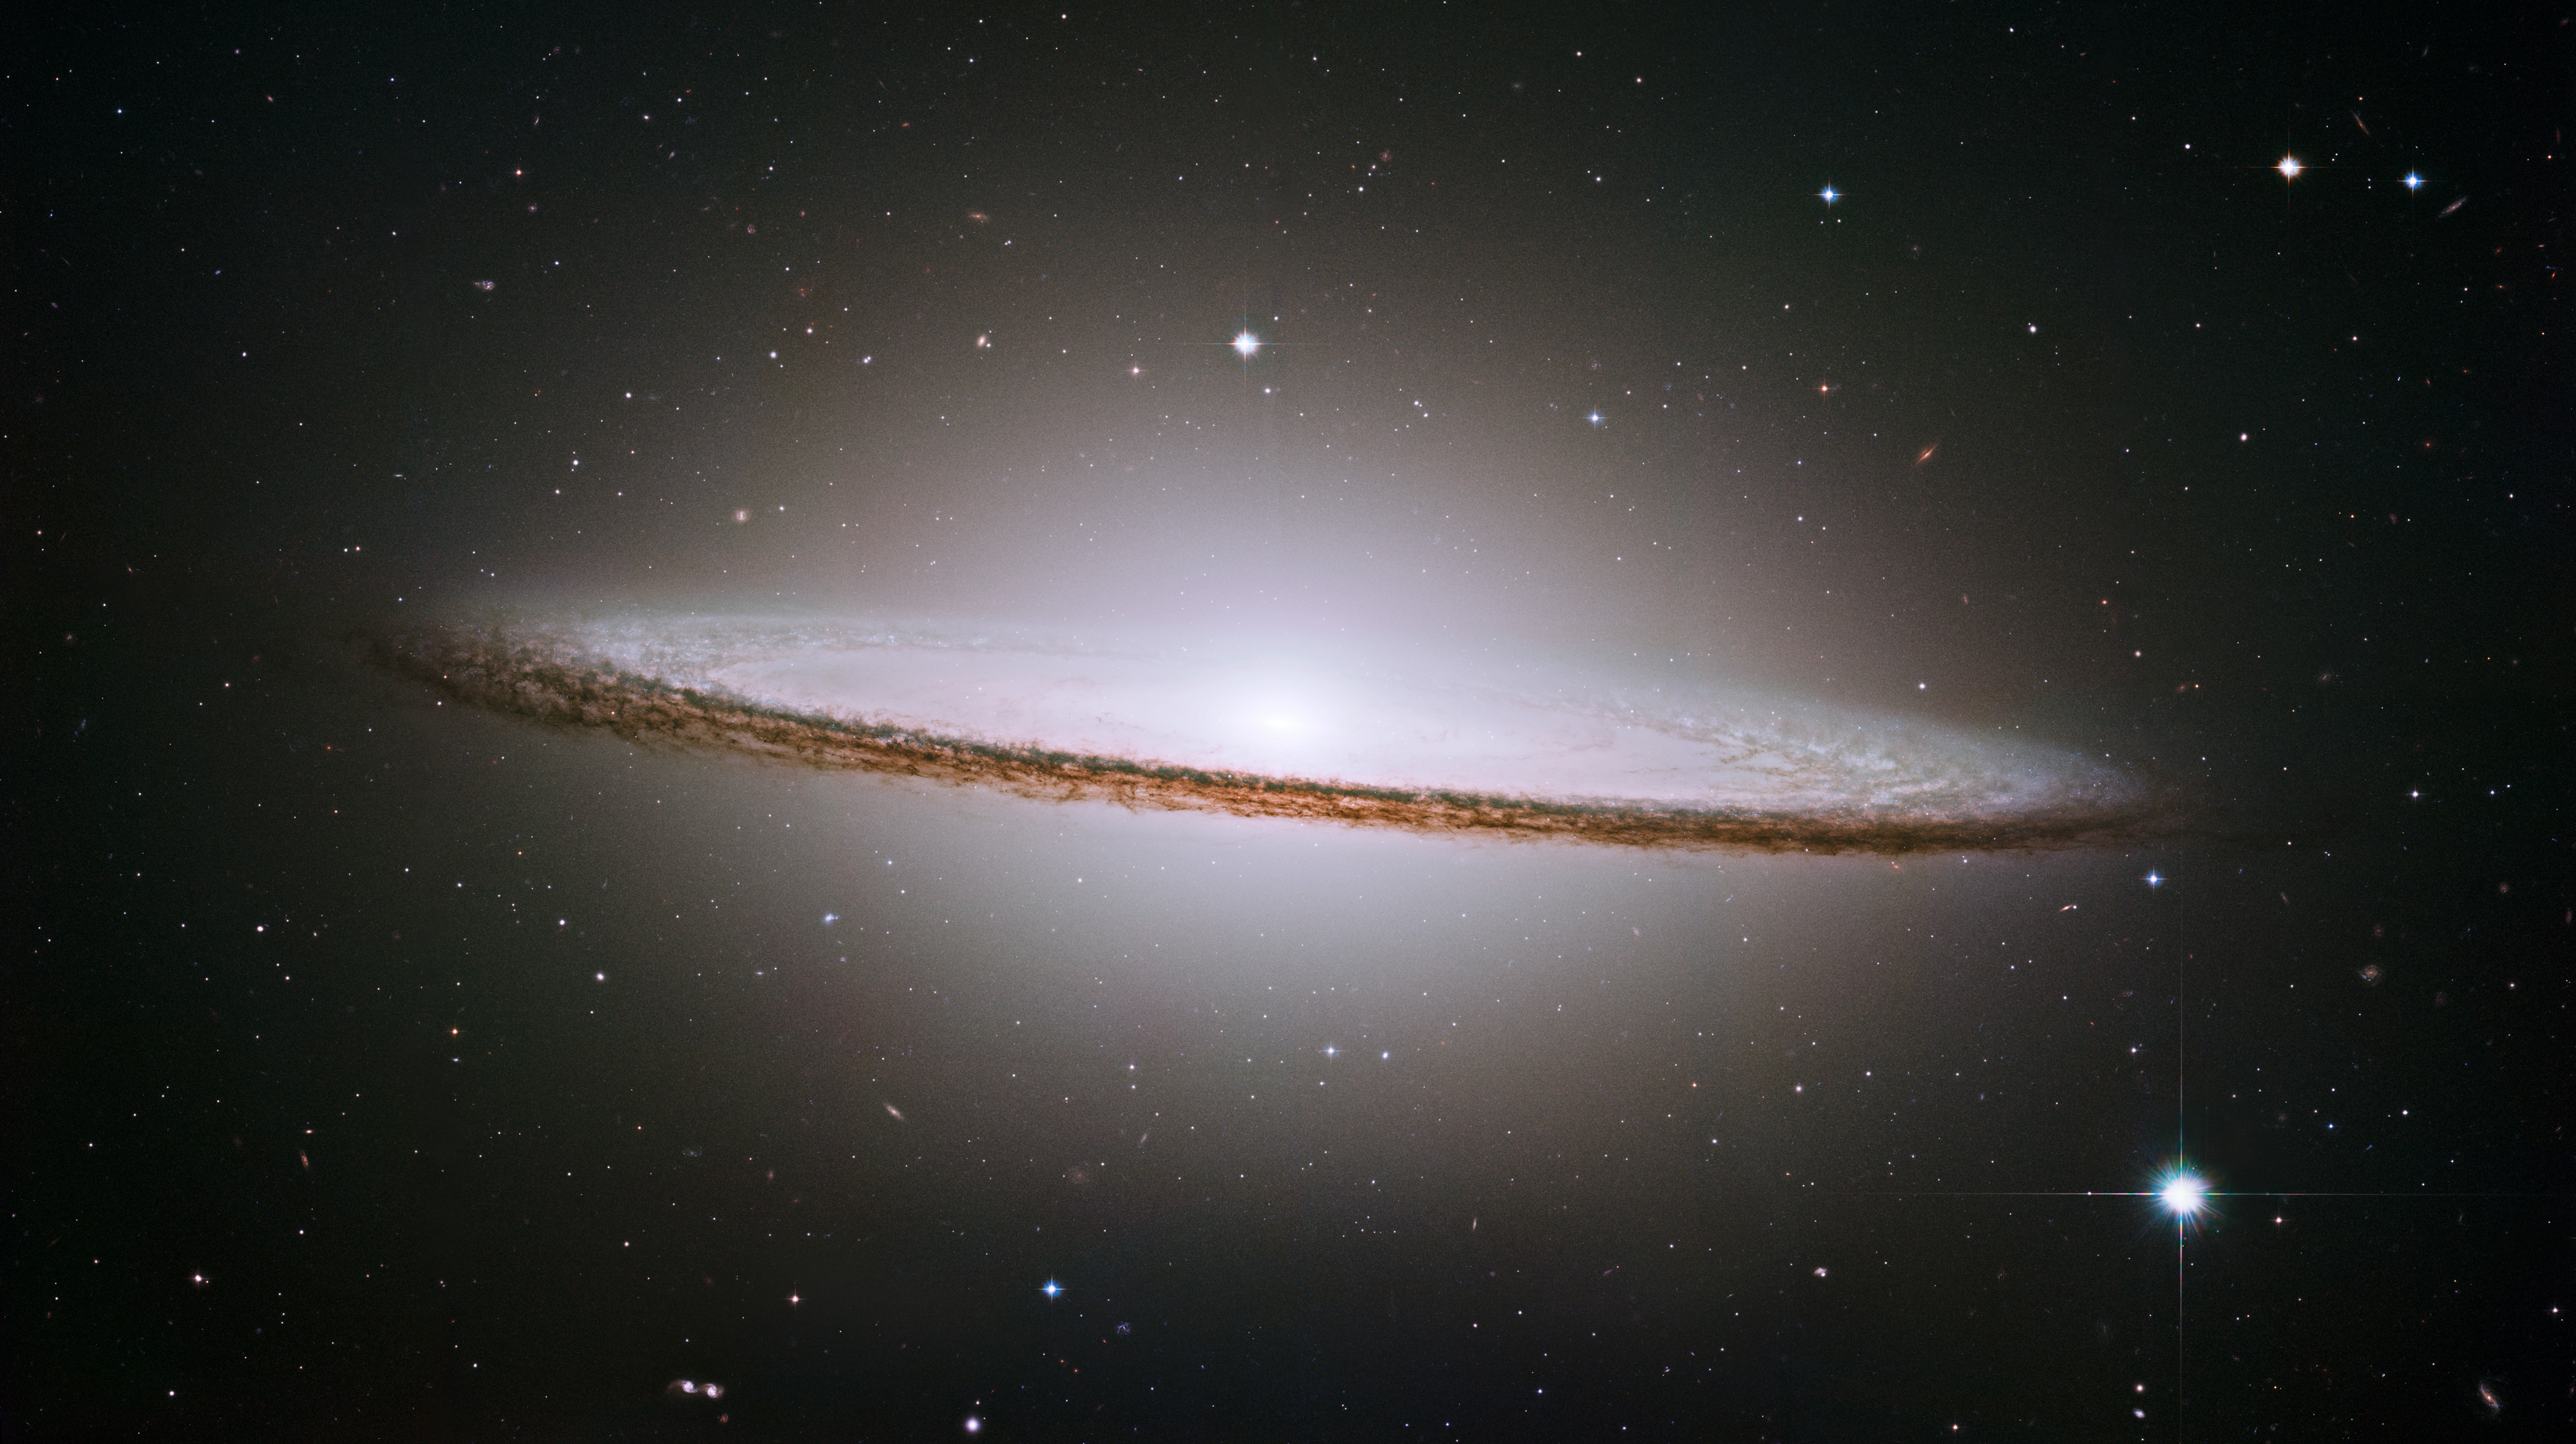
\includegraphics[width=\textwidth]{fig/1.jpg}
\caption*{Figure 1: Description details}
\end{center}
\centering
\end{figure}

\begin{algorithm}
\caption{Code Title}
\label{alg:waypointAlgo}
\begin{algorithmic}[1]
\import{}{code/1.tex}
\end{algorithmic}
\end{algorithm}


\end{document}
